
The global ledger state is stored locally by each node in a key value pair database. The choice of underlying database is arbitrary ieRocksDb, GoogleDb, however the Catalyst state  is organised using a structure called a Sparse Merkle Tree. A node using a alternative storage structure would be unable to interact with the network as they would not be able to retrieve the correct state values.
\\
\\
The Sparse Merkle Tree data structure allows for:

\begin{enumerate}
\item Persistent storage of current and previous states of the ledger.
\item Efficient provision of proof that queried data exists, or importantly, does not exist in the ledger.\end{enumerate}

\subsubsection{Merkle Tree}

A Merkle tree is a structure which allows a large set of data to be committed to with only a short string known as the root hash.  If any of the data is changed, the root hash will also change. This allows honest nodes to recognise and reject information that has been altered outside of the ledger cycle by malicious parties. 
\\
\\
Each item of data being stored (here the serialised account information) is represented as a leaf of the Merkle tree. The data in neigbouring leaves is hashed and concatenated and this value is used for the node one level above in the tree. Each node is stored in the database with its lookup key being the hash of its value. The nodes are themselves combined until a single hash has been obtained. This is the root hash and its value depends on every bit of data stored in the tree.

\begin{figure}[h]
  \centering
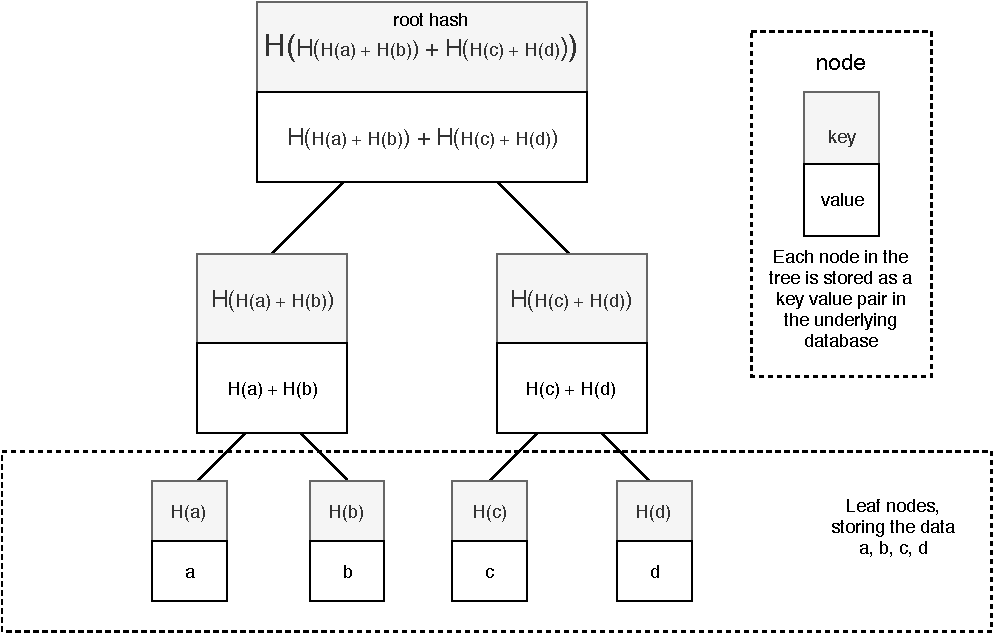
\includegraphics[scale=0.8]{merkle-tree}
\end{figure}

To store or retrieve an entry from a Merkle tree, a key is used. For the account storage we use the account address as the key. This key is not equivalent to a key in the underlying database, instead it is used to determine the path from the root hash to the data entry [ ?? is this true for non SMT???] The key tells us which branch to follow as we progress down the tree. 
\\
\\
When a data entry changes, every node above it in the tree must be recalculated. The hash of the data held by a node is used as its key in the database, therefore every recalculated node will constitute a new entry in the underlying database, rather than an existing entry that needs to be updated.

\subsubsection{Sparse Merkle Tree}

The Sparse Merkle Tree

\subsubsection{Merkle Proof}
an audit path comprises all siblings along the path down to the leaf being authenticated. Combined with a retrieved attribute, this forms a proof of membership which is valid if it reconstructs the root digest r 0 such that 

\subsubsection{Choice of Sparse Merkle Tree over Merkle Patricia Tree}

-balanced
-easy proof of non existence
-simpler to implement

